\documentclass[12pt]{article}
\usepackage{amsmath, amsfonts, amsthm, amssymb}
\usepackage{fullpage}
\usepackage{enumerate}

% For figures
\usepackage{graphicx}
\usepackage{subcaption}

\usepackage{amsmath,amssymb}

\usepackage{hyperref}

%%%%%%%%%%%%%%%%%%%%CONTENT MACROS%%%%%%%%%%%%%%%%%%%%%%%%%
\renewcommand{\qed}{\quad \ensuremath{\blacksquare}}    % QED blacksquare
\newcommand{\inv}{^{-1}}                            % inverse operator
\newcommand{\sminus}{\backslash}                    % set minus
\newcommand{\N}{\mathbb{N}}                         % natural numbers
\newcommand{\R}{\mathbb{R}}                         % real numbers
\newcommand{\pow}{\mathcal{P}}                      % power set
\newcommand{\Se}{\mathcal{S}}                       % partition
\newcommand{\D}{\mathcal{D}}                        % partition
\newcommand{\e}{\varepsilon}                        % \varepsilon
\renewcommand{\d}{\delta}                           % \delta
\newcommand{\X}{\mathcal{X}}                        % X domain
\newcommand{\Y}{\mathcal{Y}}                        % Y domain
\newcommand{\Z}{\mathcal{Z}}                        % Z domain
\newcommand{\A}{\mathcal{A}}                        % sub-domain
\newcommand{\E}{\mathbb{E}}                         % expected value
\newcommand{\V}{\mathbb{V}}                         % variance
\newcommand{\pr}{\mathbb{P}}                        % probability
\newcommand{\hP}{{\hat P}}                          % 
\newcommand{\cpest}{\widehat{p}_h}                  % clipped estimated p_n
\newcommand{\cqest}{\widehat{q}_h}                  % clipped estimated q_n
\newcommand{\pest}{\widetilde{p}_h}                 % estimated p_n
\newcommand{\qest}{\widetilde{q}_h}                 % estimated q_n
\newcommand{\dist}{\operatorname{dist}}             % distance operator
\newcommand{\acro}[1]{\textsc{\MakeLowercase{#1}}}
\newcommand{\ol}{\overline}
\renewcommand{\hat}{\widehat}
%%%%%%%%%%%%%%%%%%%%%%%%%%%%%%%%%%%%%%%%%%%%%%%%%%%%%%%%%%%

\renewcommand{\thesubsection}{\arabic{subsection}}

\usepackage{natbib}
\usepackage[disable]{todonotes}

\begin{document}
\begin{center}
{\bf\Large 37-462/662 HW 01 Solutions to Problems 1 and 2}\\
Shashank Singh\\
sss1@andrew.cmu.edu\\
\end{center}


\subsection{Problem 1}
See Figure \ref{fig:problem1} for our error plots and see Section
\ref{sec:code} for our R code. In general, long code segments should be in an
appendix rather than in the middle of your homework.
%%% BEGIN FIGURE %%%
\begin{figure}[h!]
\centering
\hfill
  \begin{subfigure}[b]{0.49\textwidth}
  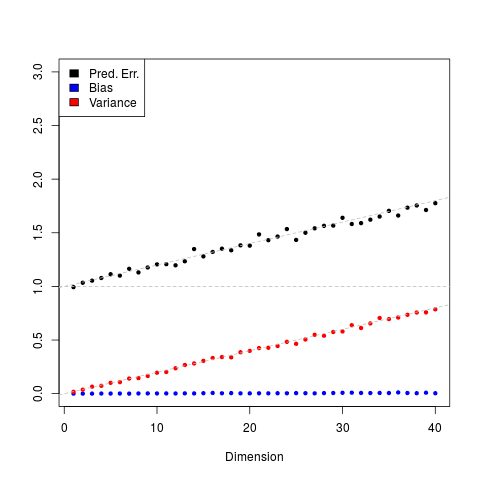
\includegraphics[width=1.05\textwidth]{linear}
  \vspace{-8mm}
  \caption{Linear Regression}
  \end{subfigure}
\hfill
  \begin{subfigure}[b]{0.49\textwidth}
  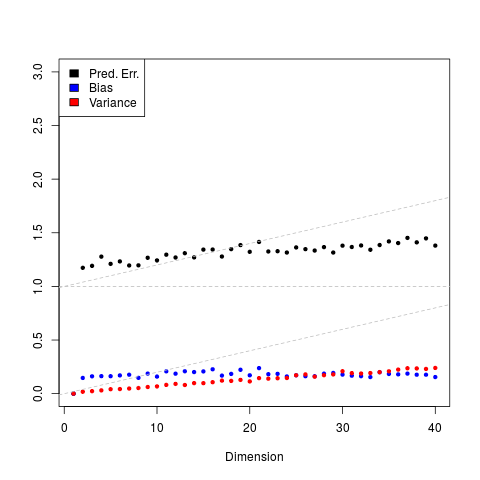
\includegraphics[width=1.05\textwidth]{ridge}
  \vspace{-8mm}
  \caption{Ridge Regression}
  \end{subfigure}
\hfill
\vspace{-2mm}
\caption{Prediction Error, Bias, and Variance for Linear and Ridge
Regression as dimension $p$ varies.}
\label{fig:problem1}
\end{figure}
%%% END FIGURE %%%

We can see that, in lower dimensions, linear regression outperforms ridge
regression (which has higher bias), but, in higher dimensions, ridge regression
peforms better by controlling the variance of linear regression. When $p = 40$,
\texttt{glmnet} chooses $\lambda \approx 26$, which is what we use here.

\newpage
\subsection{Problem 2}
\begin{enumerate}
\item[{\bf (a)}] {\bf (5 points)}
Since $Xv = 0$, for any $c \in \R$,
\[\|y - X(\hat\beta + c \cdot v)\|_2^2
    = \|y - X\hat\beta + c \cdot Xv\|_2^2
    = \|y - X\hat\beta + c \cdot \vec 0\|_2^2
    = \|y - X\hat\beta\|_2^2.
\]
Hence, $\hat\beta + c \cdot v$ has the same least squares loss as $\hat\beta$
and is also a minimizer.

\item[{\bf (b)}] {\bf (5 points)}
Since $Xv = v_1 \cdot x_1 + \dots + v_p \cdot x_p$ is a linear combination of
the linearly independent set $\{x_1,\dots,x_p\}$ with coefficients
$v_1,\dots,v_p$, $Xv = 0$ implies $v = 0$.
\footnote{
{\bf Technical Note:} Several students claimed that, because $X$ has linearly
independent columns, it has an inverse $X\inv$. Only square matrices have
proper inverses, with $XX\inv = I = X\inv X$. What is true here is that $X$ has
a \emph{left inverse} $X\inv$ with $X\inv X = I$ (but not $XX\inv = I$). In
this case, a left inverse is all we need, but not making this distinction can
sometimes lead one to derive false statements.}

{\bf Note:} This tells us that least squares regression is safe (or at
least well-defined) when our samples span $\R^p$. However, this can only happen
when we have at least $p$ samples.

\item[{\bf (c)}] {\bf (15 points)} Because $Xv$ is a linear combination of $p$
column vectors in $\R^n$, if $p > n$, the columns of $X$ are linearly
dependent. Thus, there exists a particular $v \neq 0$ such that $Xv = 0$.
\footnote{Another valid way to phrase this is that the homogeneous linear
system $Xv = 0$ has more variables than equations, and hence has a nonzero
solution $v \neq 0$. You should understand both explanations.}

If we let $\hat\beta$ be a linear regression estimate (i.e., a least-squares
minimizer), part (a) then tells us that, for any of the infinitely many
$c \in \R$, $\hat\beta' = \hat\beta + c \cdot v$, is also a valid linear
regression estimate.

Since $v \neq 0$, some component $v_i \neq 0$, and so, for any $r \in \R$, if
we choose $c = \frac{r - \hat\beta_i}{v_i}$, then
$\hat\beta_i' = \hat\beta_i + c v_i = r$. Thus, $\hat\beta_i'$ could be any
real number, and so we have no way to interpreting the dependence of $y$ on the
covariate $x_i$ in our model.

{\bf Note:} An intuitive way to view this is that each sample imposes a linear
constraint on the $p$-dimensional variable $\beta$ that encodes our model.
Thus, when $p > n$, we have insufficient data to specify the model, suggesting
the need for other constraints (such as a regularization term).
\end{enumerate}

\newpage
\subsection{Code Appendix}
\label{sec:code}

\begin{verbatim}
# if you don't already have glmnet installed, run
# install.packages("glmnet", repos = "http://cran.us.r-project.org")
library(glmnet)
n = 50; p_max = 40; ridge_lambda = 1
reps = 100 # number of trials

## Comment one out
method = "linear" #For linear regression
# method = "ridge" #For ridge regression
bias = numeric(p_max); variance = numeric(p_max); pred_err = numeric(p_max)

for (p in 1:40){
  # Skip p=1 in ridge regression because glmnet fails
  if (method=='ridge' && p==1){next}

  X = matrix(rnorm(n*p),ncol=p) # n normal random covariate samples in R^p
  beta = c(1,runif(p-1,-.2,.2)) # beta_1 = 1 and other betas uniformly random
  y_hat = matrix(0,nrow=n,ncol=reps)
  y_prime = matrix(0,nrow=n,ncol=reps)

  for (k in 1:reps){
    y_train = X%*%beta + rnorm(n) # y = X*beta + noise

    if (method=='linear'){
      # lsfit is convenient; important to not include intercept here
      beta_hat = lsfit(X,y_train,intercept=FALSE)$coef
    } else if (method=='ridge') {
      # glmnet returns a sparse vector with an intercept entry, even when the
      # intercept is excluded; this extracts the correct entries as numeric
      beta_hat = as.numeric(coef(
                    glmnet(X,y_train,intercept=FALSE,alpha=0,family='gaussian'),
                s=ridge_lambda)[2:(p+1)])
    }

    y_hat[,k] = X%*%beta_hat # true y
    y_prime[,k] = X%*%beta + rnorm(n) # predicted y
  }
  pred_err[p] = mean((y_prime-y_hat)^2)
  bias[p] = mean((X%*%beta-rowMeans(y_hat))^2)
  variance[p] = mean((y_hat-rowMeans(y_hat))^2)
}
# plot error for each p
plot(1:p_max,pred_err,col='black',ylim=c(0,3),pch=20,xlab="Dimension",ylab="")
points(1:p_max,bias,col='blue',pch=20)
points(1:p_max,variance,col='red',pch=20)

# plot trend lines
abline(a=0,b=1/n,lty=2,col='grey')
abline(a=1,b=1/n,lty=2,col='grey')
abline(h=1,lty=2,col='grey')

legend('topleft',legend=c("Pred.Err.","Bias","Variance"),fill=c('black','blue',
                                                                        'red'))
\end{verbatim}

%{\small
%\bibliography{biblio}
%%\bibliographystyle{icml2014}
%\bibliographystyle{plain}
%}
\end{document}
